
Figure~\ref{fig:mjj} presents the \mjj spectra in the \lllljj and \llvvjj SRs, as well as in the \lllljj QCD $ZZjj$ CR,
where the normalization of the $ZZjj$ processes is fixed to the observed value, as explained later in this section.
This figure
%shows a good agreement between the data and the predictions,
indicates the high \mjj region as the most sensitive to EW $ZZjj$ event detection.
Figure~\ref{fig:mZZ} depicts the invariant mass of the four-lepton system ($m_{ZZ}$) in the \lllljj channel.
%The $m_{ZZ}$ is a sensitive variable to probe EWSB and that we start to be sensitive to the TeV scale.

To separate the EW $ZZjj$ processes from their backgrounds, MDs based on the Gradient Boosted Decision Tree algorithm~\cite{friedman2001} are trained with simulated events using the TMVA framework~\cite{Hocker:2007ht}. In each channel, a single MD is trained in the SR, which uses event kinematic information sensitive to the characteristics of the EW signal. In the \lllljj channel, twelve input variables are used: \mjj, \dyjj, \pt~of the leading and subleading jets (\ptleadj and \ptsubj), product of jet rapidities ($y_{j1}\times y_{j2}$), \pt~of the $Z$ boson reconstructed from the lepton pair with the mass closer to the $Z$ boson mass, rapidity of both $Z$ bosons ($y_{Z1}$ and $y_{Z2}$), \pt~and mass of the four-lepton system, \pt~of the third lepton, \pt~of the $ZZjj$ system divided by the scalar \pt~sum of $Z$ bosons and two jets ($S_{\mathrm{T}}$). Thirteen input variables are utilized in the \llvvjj channel, which are \mjj, \dyjj, $y_{j1}\times y_{j2}$, \ptsubj, \met, \met~significance, $S_{\mathrm{T}}$, pseudorapidity and azimuthal angle difference between two leptons ($\Delta\eta$, $\Delta\phi$), $\Delta R = \sqrt{(\Delta\eta)^2 + (\Delta\phi)^2}$, invariant mass of the lepton pair, and \pt~of leading and subleading leptons.
%The different set of variables in the \llvvjj channel is chosen in light of the presence of \nonresll~and $WZjj$ backgrounds, in addition to the irreducible QCD $ZZjj$ process.
The jet-related information provides the greatest sensitivity in the \lllljj channel, while both the jet-related and the dilepton-related variables are important in the \llvvjj channel. 

In the \lllljj channel the MD distributions in both the SR and the QCD $ZZjj$ CR are used in the statistical fit,
while only the MD distribution in the SR is fitted in the \llvvjj channel.
The yields of the background processes in the \llvvjj channel are determined in the CRs in data and are subsequently fixed in the statistical fit.
Figure~\ref{fig:MVA_2l2v_CR} presents the observed and predicted MD distributions in the $WZjj$ CR in the \llvvjj channel, where the predictions and the data are found to be compatible. 

To examine the compatibility of the data and the signal-plus-background hypothesis, a test statistic is defined using the profile likelihood ratio method~\cite{cowan:Asymptotic2013}.  The likelihood function is the product of all the Poisson probability density functions built in individual MD bins and across all the regions, including the \lllljj and \llvvjj SRs and the \lllljj QCD $ZZjj$ CR. In each bin the observed number of events in data is represented by a Poisson probability density function with a mean equal to the sum of the predicted signal and background yields. The systematic uncertainties are implemented as nuisance parameters (NPs) constrained by auxiliary Gaussian functions. In most cases, a common NP is used to account for each systematic uncertainty in all the bins and regions. The statistical uncertainties of the simulated samples are uncorrelated among all bins, and the background uncertainties only apply to the corresponding backgrounds. The theoretical uncertainties for the $ZZjj$ production are uncorrelated between the \lllljj and \llvvjj channels, due to the different fiducial volume definitions. The QCD scale uncertainty for QCD $ZZjj$ production is treated as uncorrelated between the SR and the QCD CR in the \lllljj channel, as the two regions are selected with a large phase-space difference. Furthermore, two separate NPs are implemented to account for the generator modelling uncertainty for QCD $ZZjj$ production in the low and high MD regions.

The binning of MD distributions in the SRs is optimised to maximise the sensitivity of detecting EW $ZZjj$ events.
In the \lllljj channel, the normalisation of QCD $ZZjj$ production (\muQCD) is varied simultaneously in the fit in the SR and QCD CR.
The measured fiducial cross-section over the SM prediction for EW $ZZjj$ production (\muEW) is taken as the parameter of interest.
The effects of the uncertainties associated to normalizations and shapes of background processes in the MD distribution
are taken into account, except for theoretical uncertainties associated to the EW signal normalization,
so that the uncertainty in the fitted \muEW~directly corresponds to that in the measured fiducial cross-section.
The statistical tests are performed in both the individual \lllljj and \llvvjj channels, and in the combined channel.
The results are shown in Table~\ref{tab:fit_result}. 
To build the test statistic and derive the expected results, observed data is used in the QCD $ZZjj$ CR in the \lllljj channel,
while in the SRs Asimov datasets are constructed from the SM predictions with \muEW $=1$ and \muQCD $=1$ in both the \lllljj and \llvvjj channels.
From the combined channel, the observed \muEW is $1.35\pm0.34$, while \muQCD is determined to be $0.96\pm0.22$.
The total systematic uncertainty in \muEW is about 0.1, while the data statistical uncertainty is 0.3.
The background-only hypothesis is rejected at 5.5 $\sigma$ (4.3 $\sigma$) from the data (expectation), leading to the observation of EW $ZZjj$ production. 
The post-fit MD distributions are shown in Figure~\ref{fig:MVA}.
The EW $ZZjj$ cross-section (combing the \lllljj and \llvvjj channels) in the fiducial volume is derived to be $0.82\pm0.21$ fb, 
calculated as \muEW multiplied by the SM prediction of $0.61 \pm 0.03$ fb.

\begin{table}[!htbp]
\begin{center}
\begin{tabular}{c|c|c|c}
\hline
                 & $\mu_{\mathrm{EW}}$ &  $\mu^{\ell\ell\ell\ell jj}_{\mathrm{QCD}}$   &  Significance Obs. (Exp.) \\
\hline
\lllljj          & $1.54 \pm 0.42$     &  $0.95 \pm 0.22$                              &  5.48 (3.90) $\sigma$     \\
\hline
\llvvjj          & $0.73 \pm 0.65$     &  -                                            &  1.15 (1.80) $\sigma$     \\
\hline
Combined         & $1.35 \pm 0.34$     &  $0.96 \pm 0.22$                              &  5.52 (4.30) $\sigma$     \\
\hline
\end{tabular}
\end{center}
\caption{
Observed \muEW and \muQCD, as well as the observed and expected significance from the individual \lllljj and \llvvjj channels, and the combined fits.
The full set of systematic uncertainties is included.
}
\label{tab:fit_result}
\end{table}


\begin{figure}[!htbp]
\begin{center}
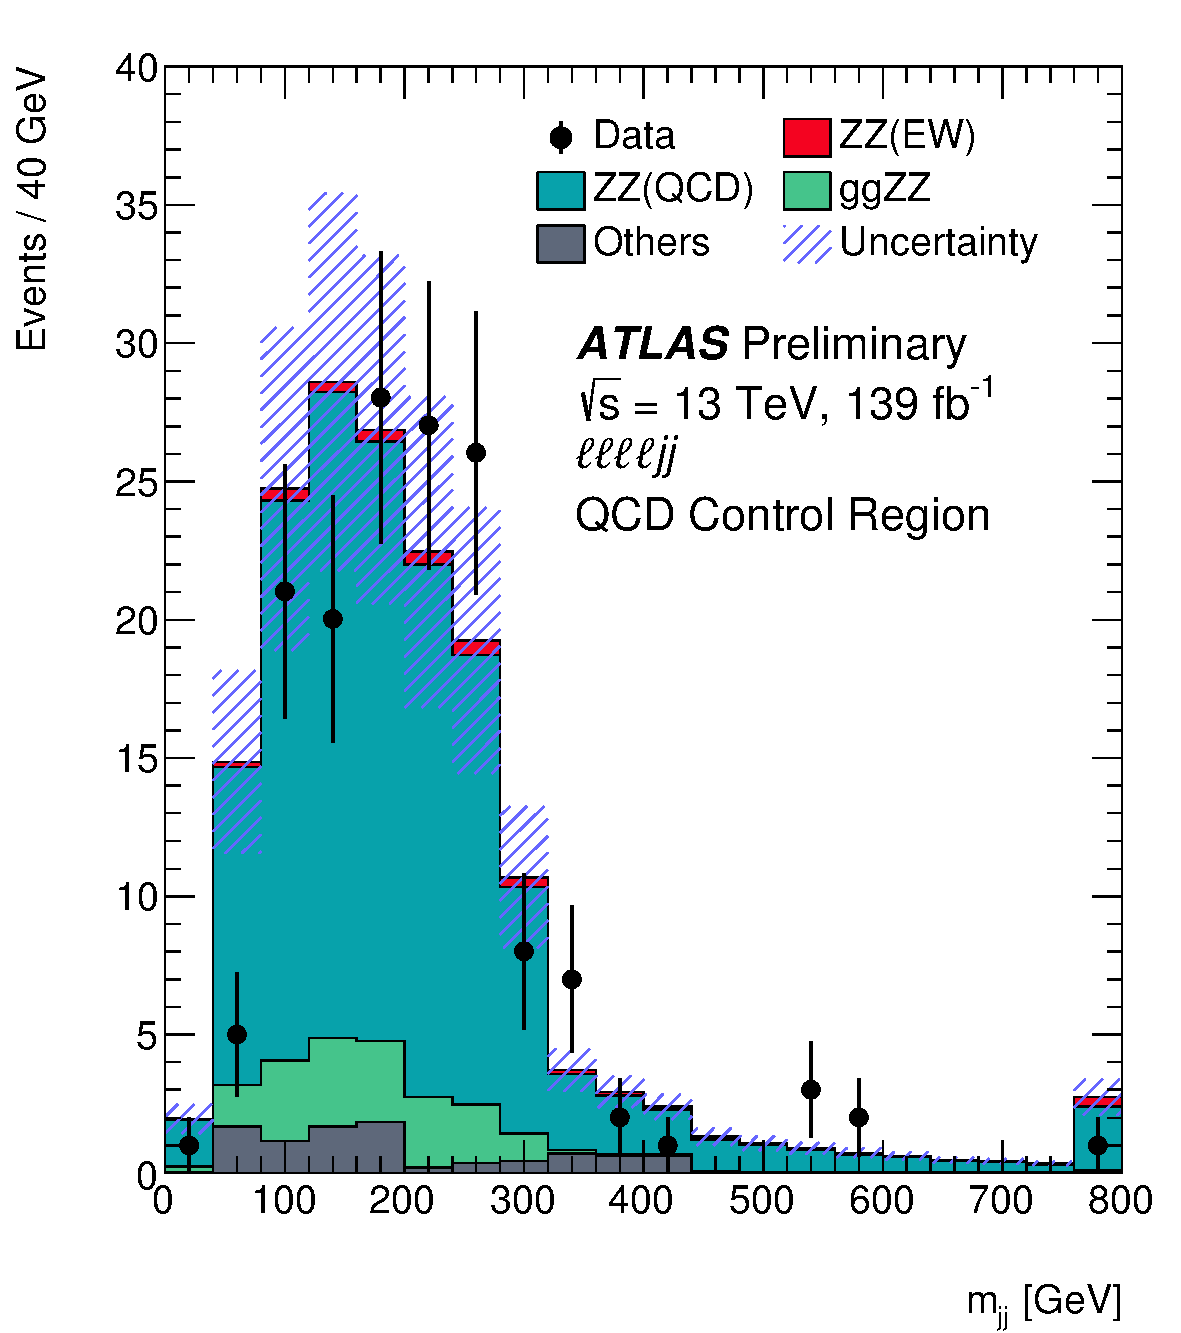
\includegraphics[width=0.325\textwidth]{figures/4l/MJJ_4l_QCD_CR_v1.pdf}
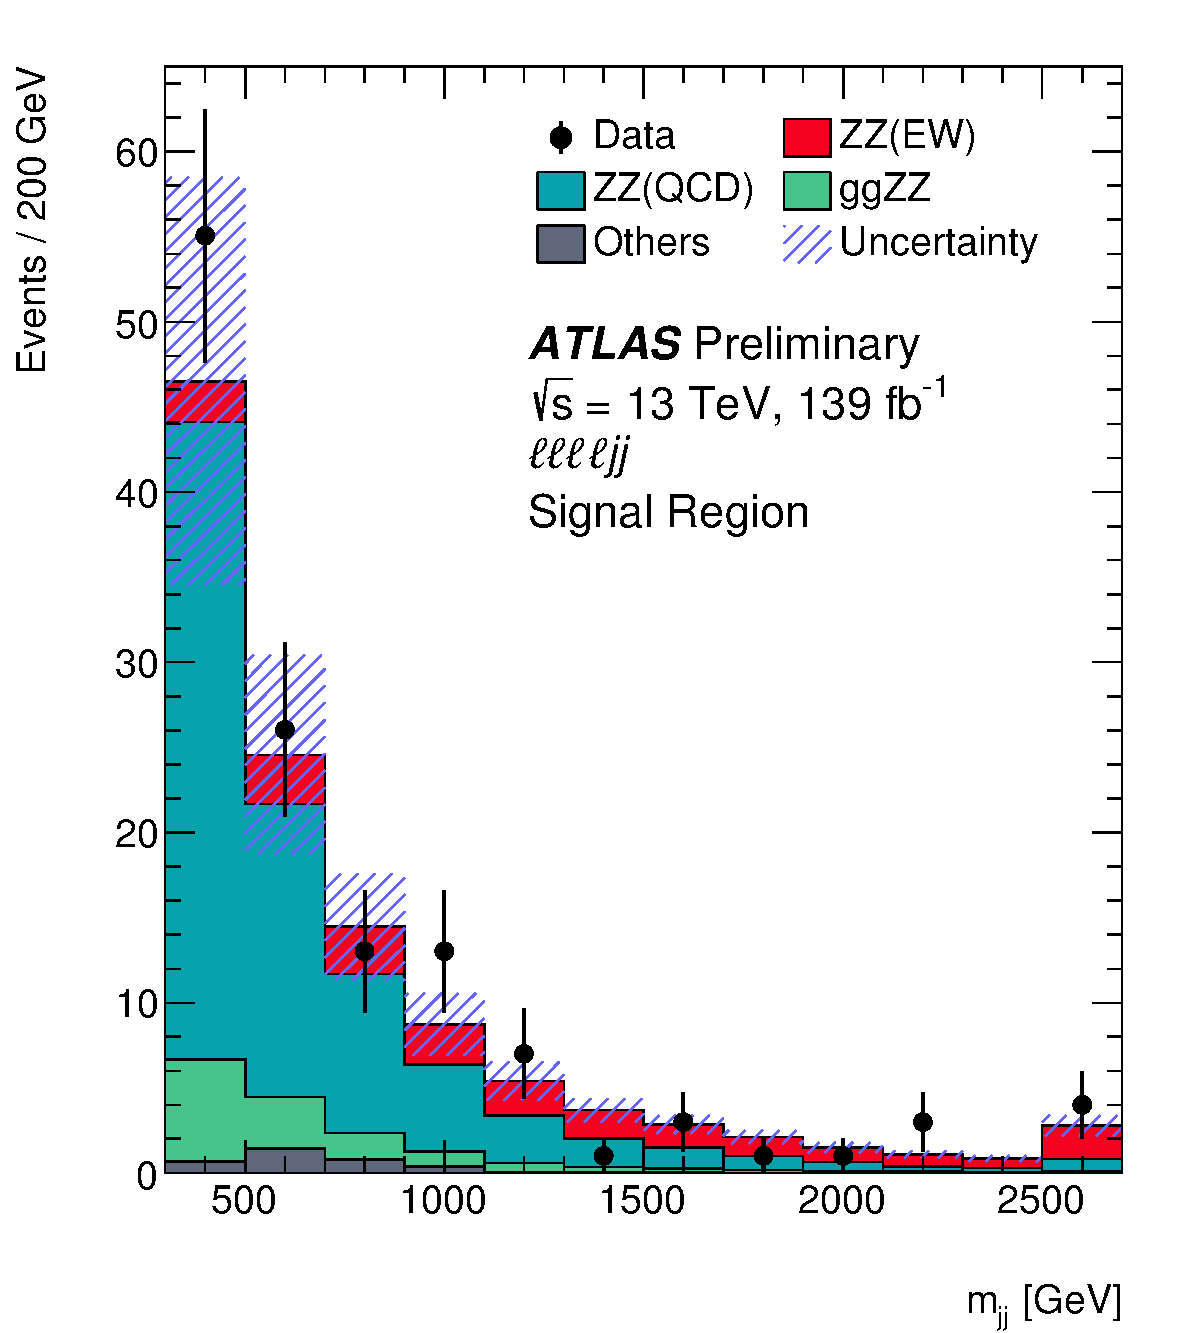
\includegraphics[width=0.325\textwidth]{figures/4l/MJJ_4l_SR_v1.pdf}
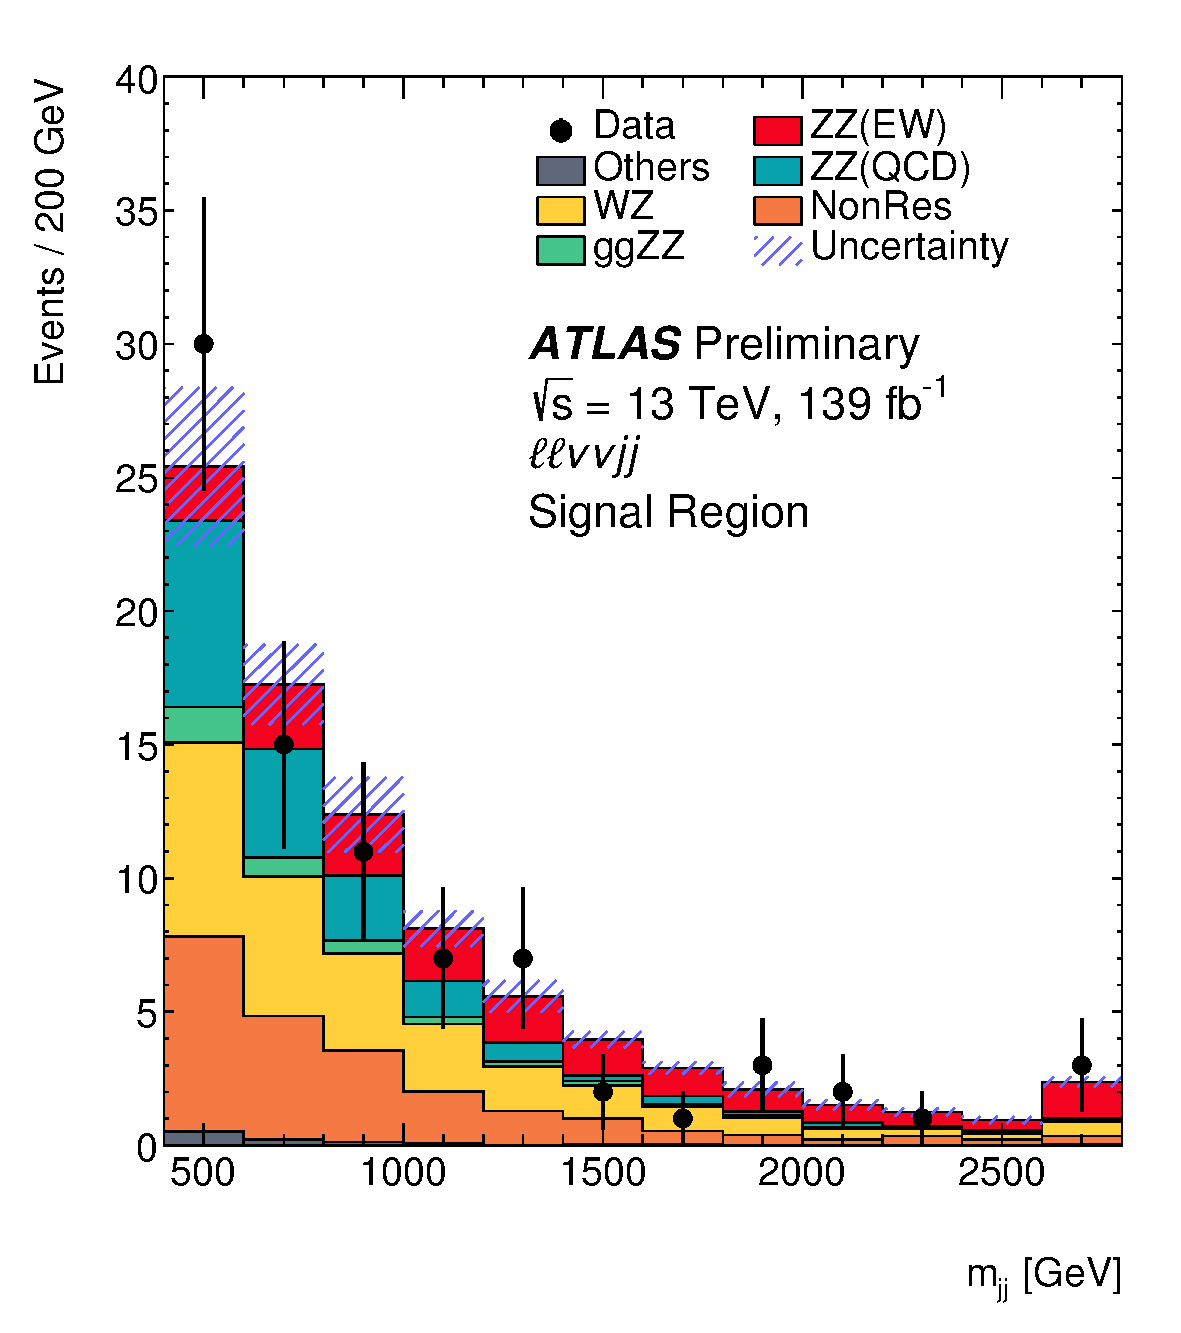
\includegraphics[width=0.325\textwidth]{figures/llvv/MJJ_2l2v_SR_v1.pdf}\\
\end{center}
\caption{Observed and expected \mjj distributions in the \lllljj QCD CR (left), 
        and in the \lllljj (middle) and \llvvjj (right) signal regions.
        The error bands include the expected experimental and theoretical uncertainties.
        The error bars on the data points show the statistical uncertainty on data.
        The contributions from the QCD and EW production of $ZZjj$ events are scaled by 0.96 and 1.35, respectively, 
        which correspond to the observed normalization factors in the statistical fit to the combined channel.
        The last bin includes the overflow events.
        }
\label{fig:mjj}
\end{figure}

\begin{figure}[!htbp]
\begin{center}
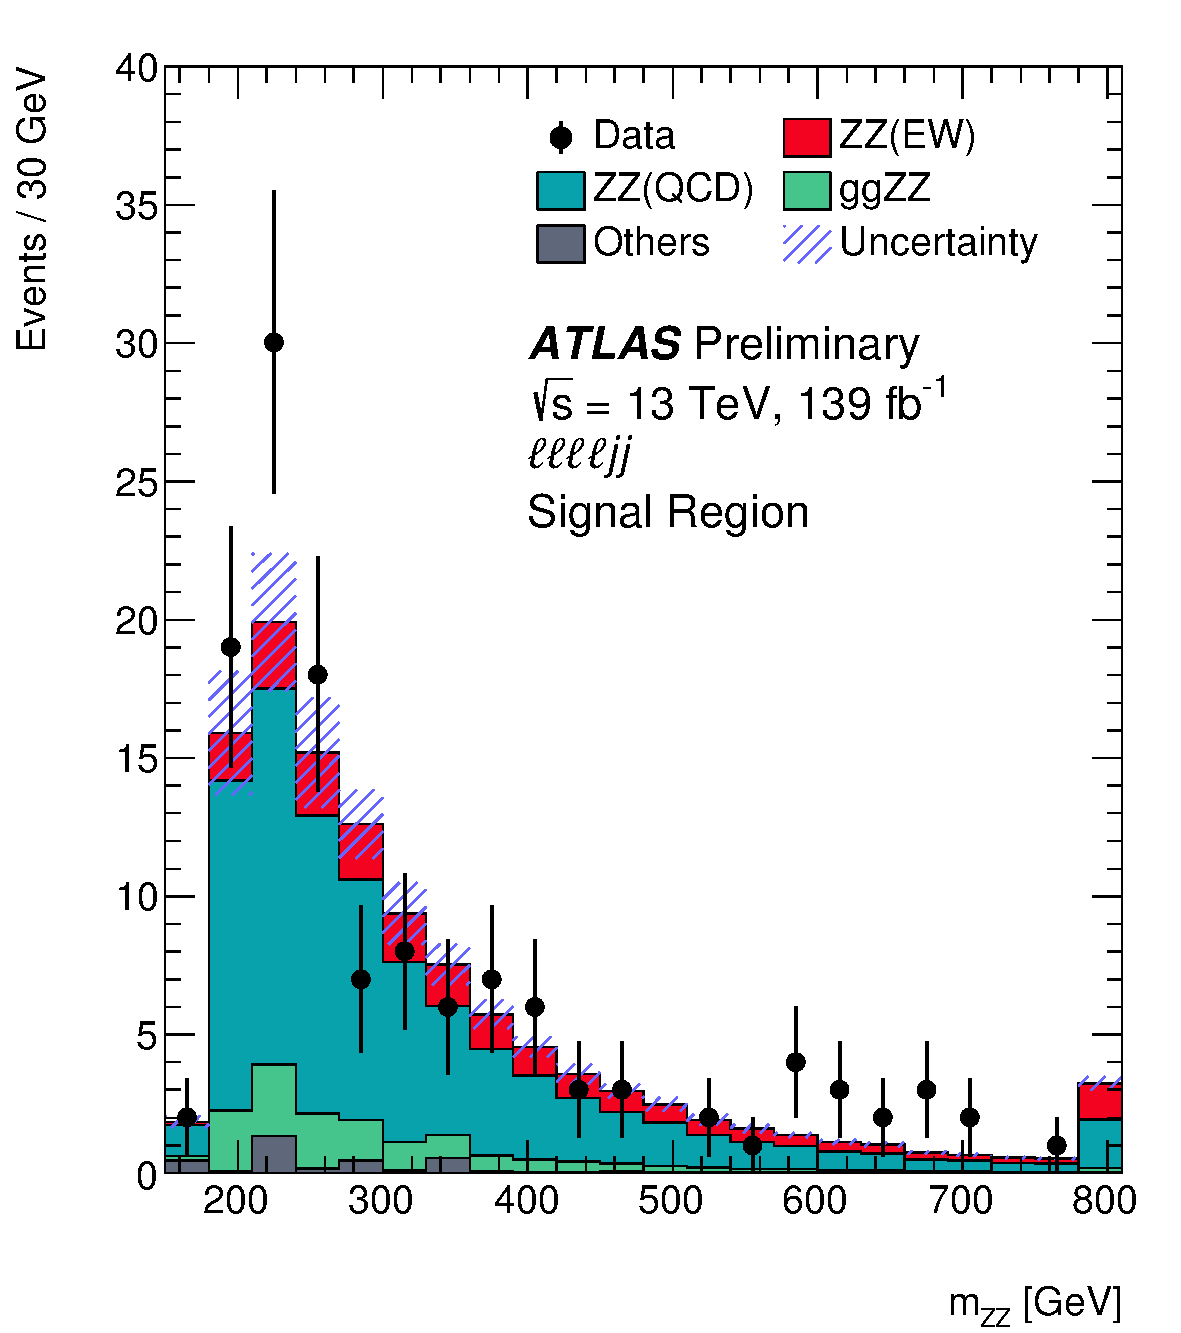
\includegraphics[width=0.4\textwidth]{figures/4l/MZZ_4l_SR_v1.pdf} \\
\end{center}
\caption{Observed and expected $m_{ZZ}$ distributions in the \lllljj channel SR. 
        The error bands include the expected experimental and theoretical uncertainties.
        The error bars on the data points show the statistical uncertainty on data.
        The contributions from the QCD and EW production of $ZZjj$ events are scaled by 0.96 and 1.35, respectively, 
        which correspond to the observed normalization factors in the statistical fit to the combined channel.
        The last bin includes the overflow events.
        }
\label{fig:mZZ}
\end{figure}

\begin{figure}[!htbp]
\begin{center}
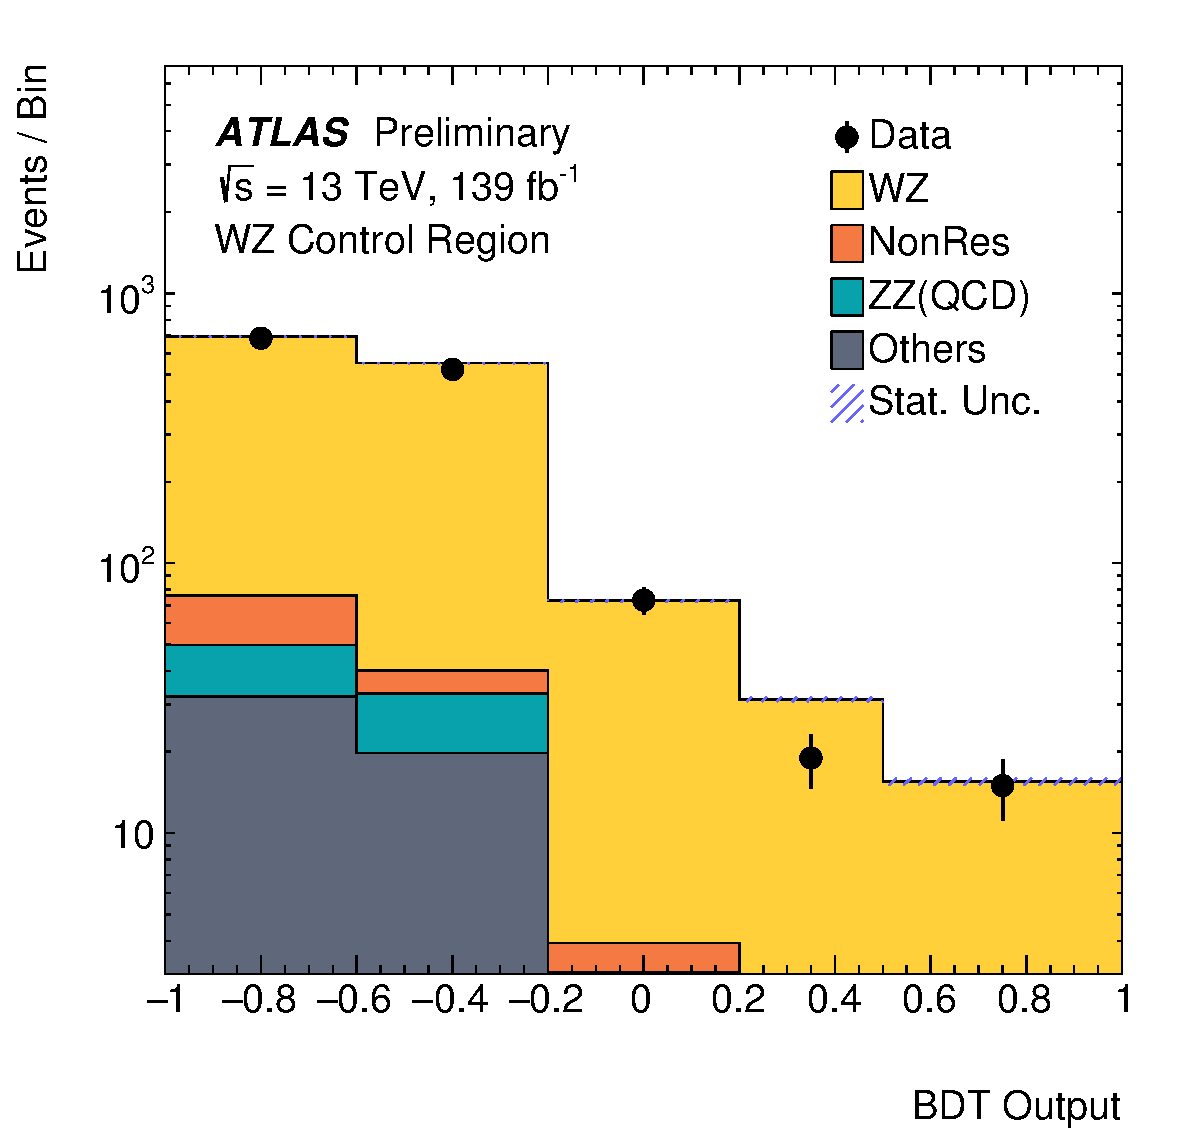
\includegraphics[width=0.4\textwidth]{figures/llvv/BDT_2l2v_3lCR.pdf} \\
%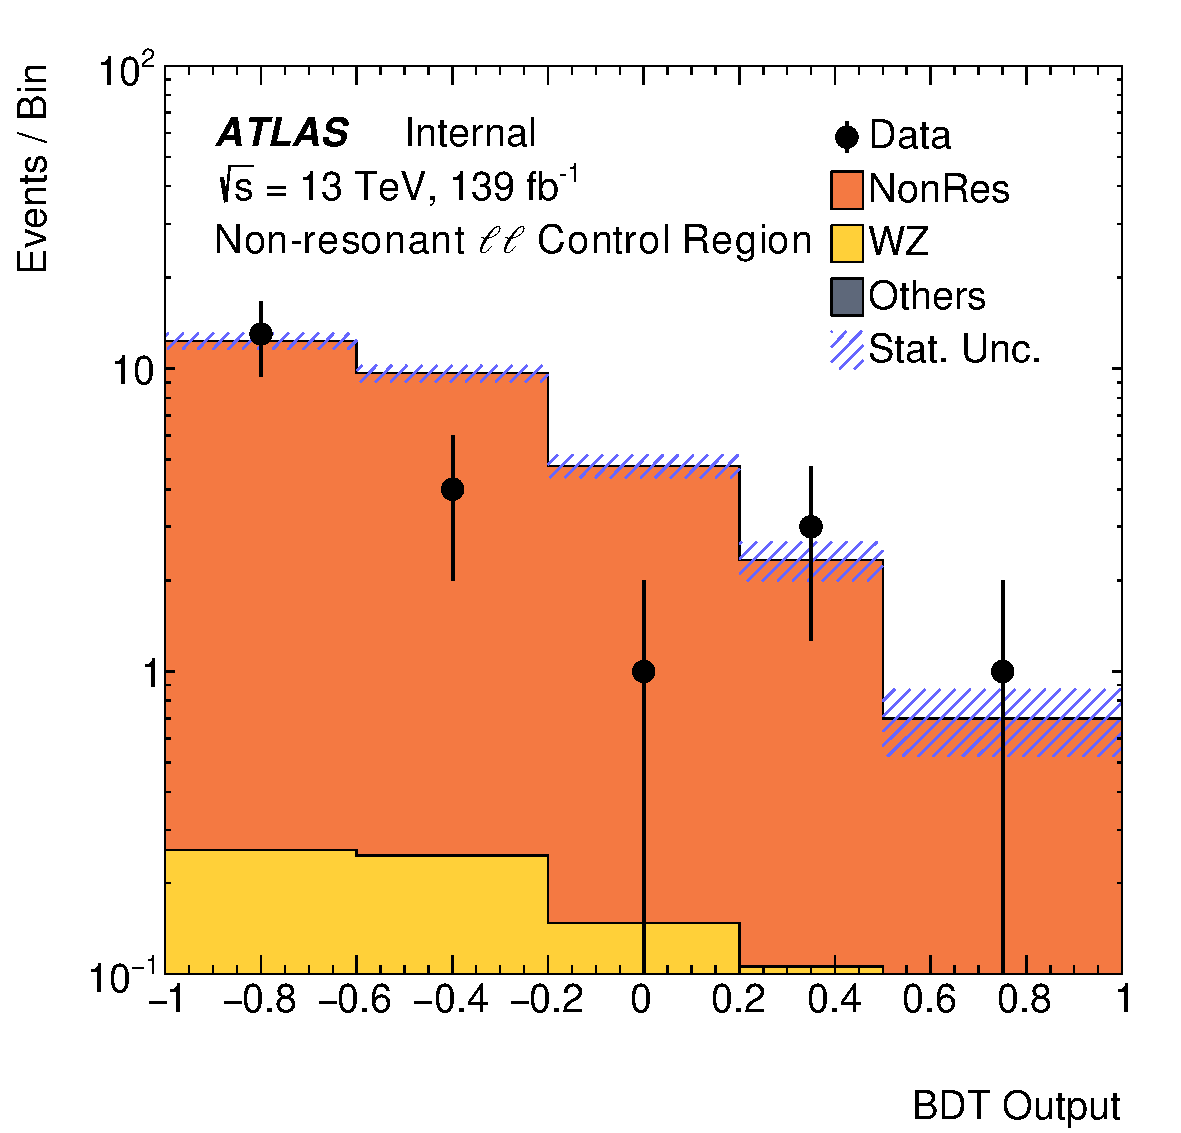
\includegraphics[width=0.325\textwidth]{llvv/BDT_2l2v_emCR.pdf} \\
\end{center}
\caption{Observed and expected multivariate discriminant distributions in the \llvvjj channel for 
        the $WZjj$
        %(left) and \nonresll (right)
        control region.
        The error bands only include the statistical uncertainties of the simulated samples.
        The error bars on the data points show the statistical uncertainty on data.
        }
\label{fig:MVA_2l2v_CR}
\end{figure}

\begin{figure}[!htbp]
\begin{center}
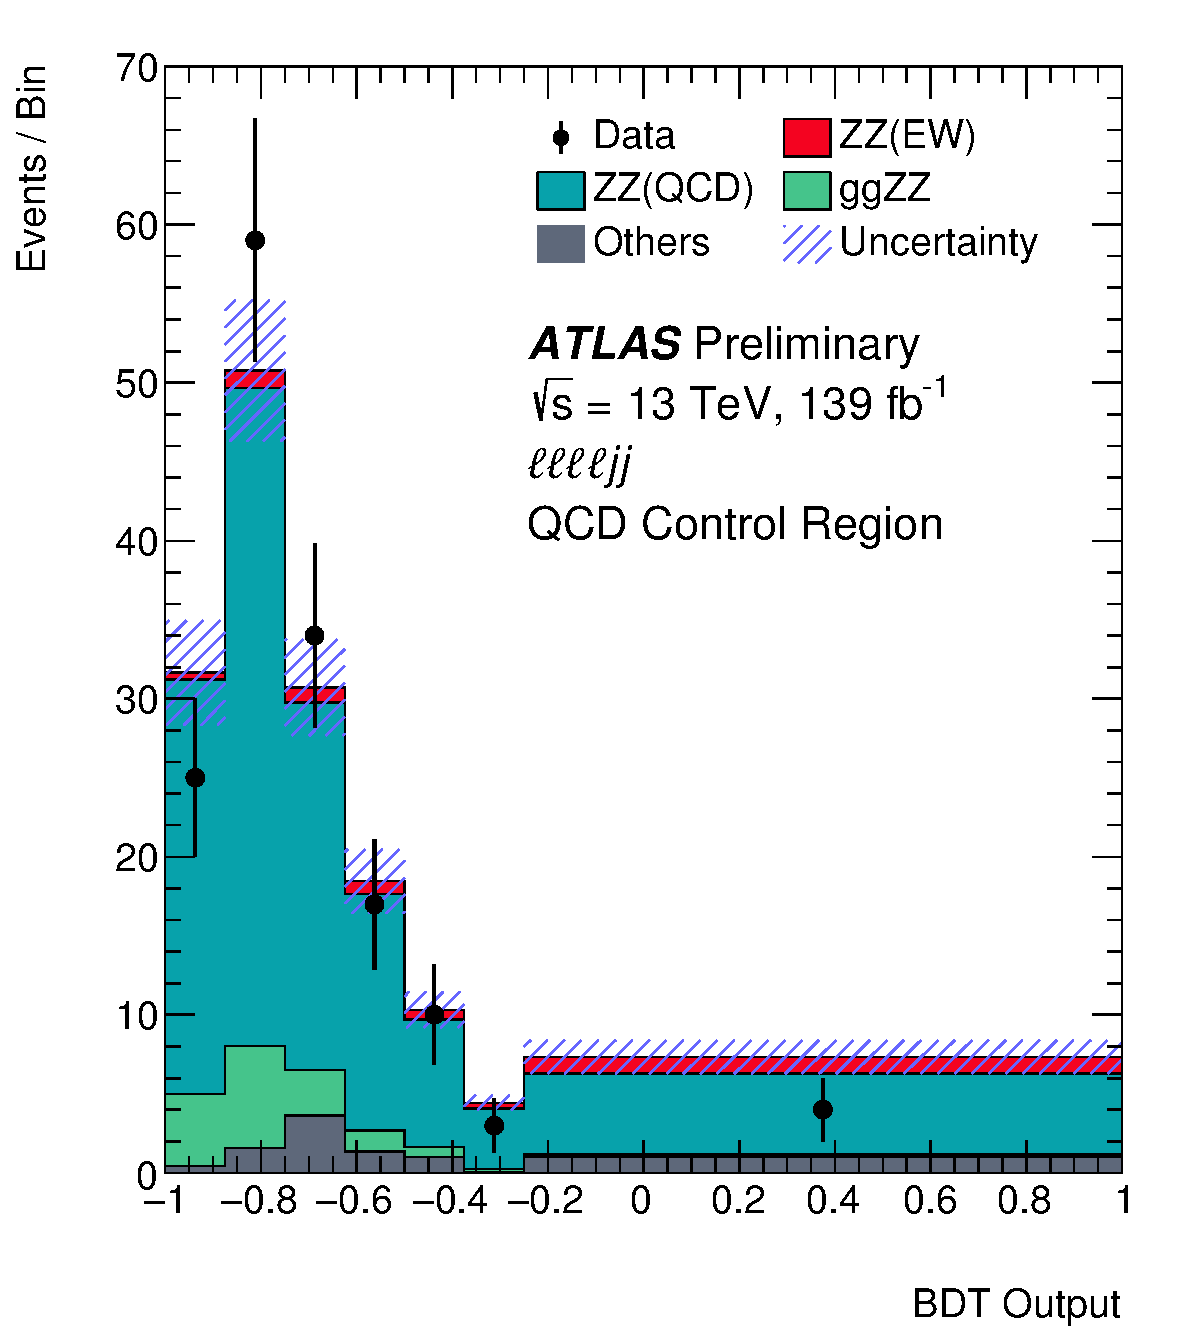
\includegraphics[width=0.325\textwidth]{figures/4l/BDT_4l_QCD_CR_postFit_v1.pdf}
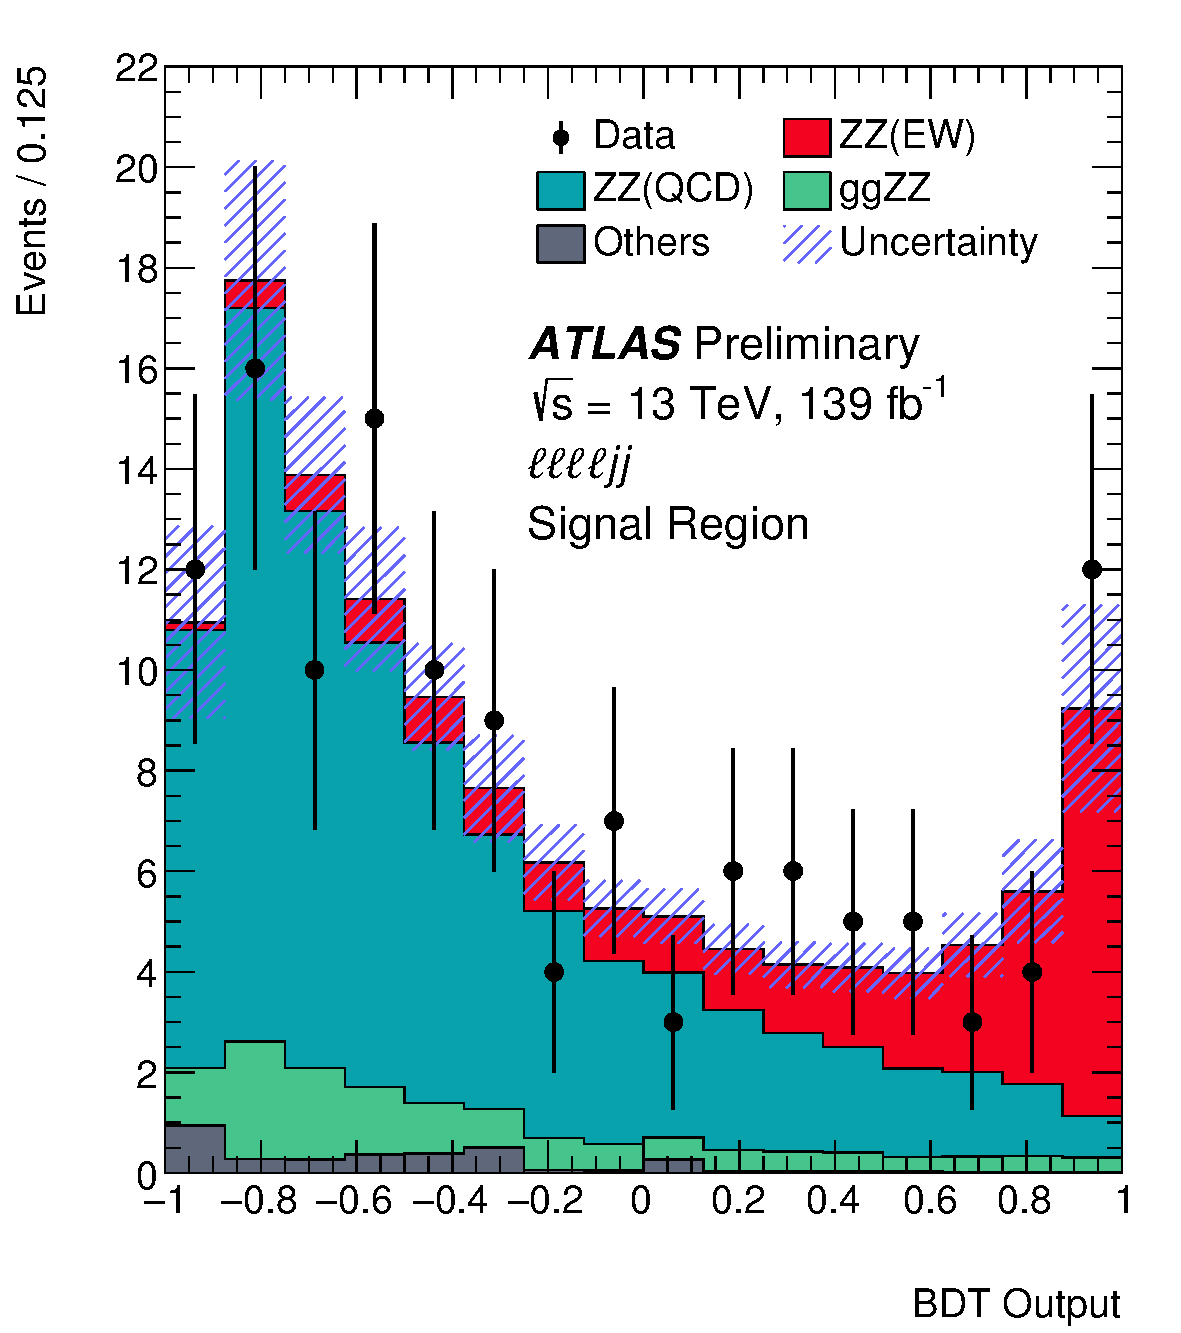
\includegraphics[width=0.325\textwidth]{figures/4l/BDT_4l_SR_postFit_v1.pdf}
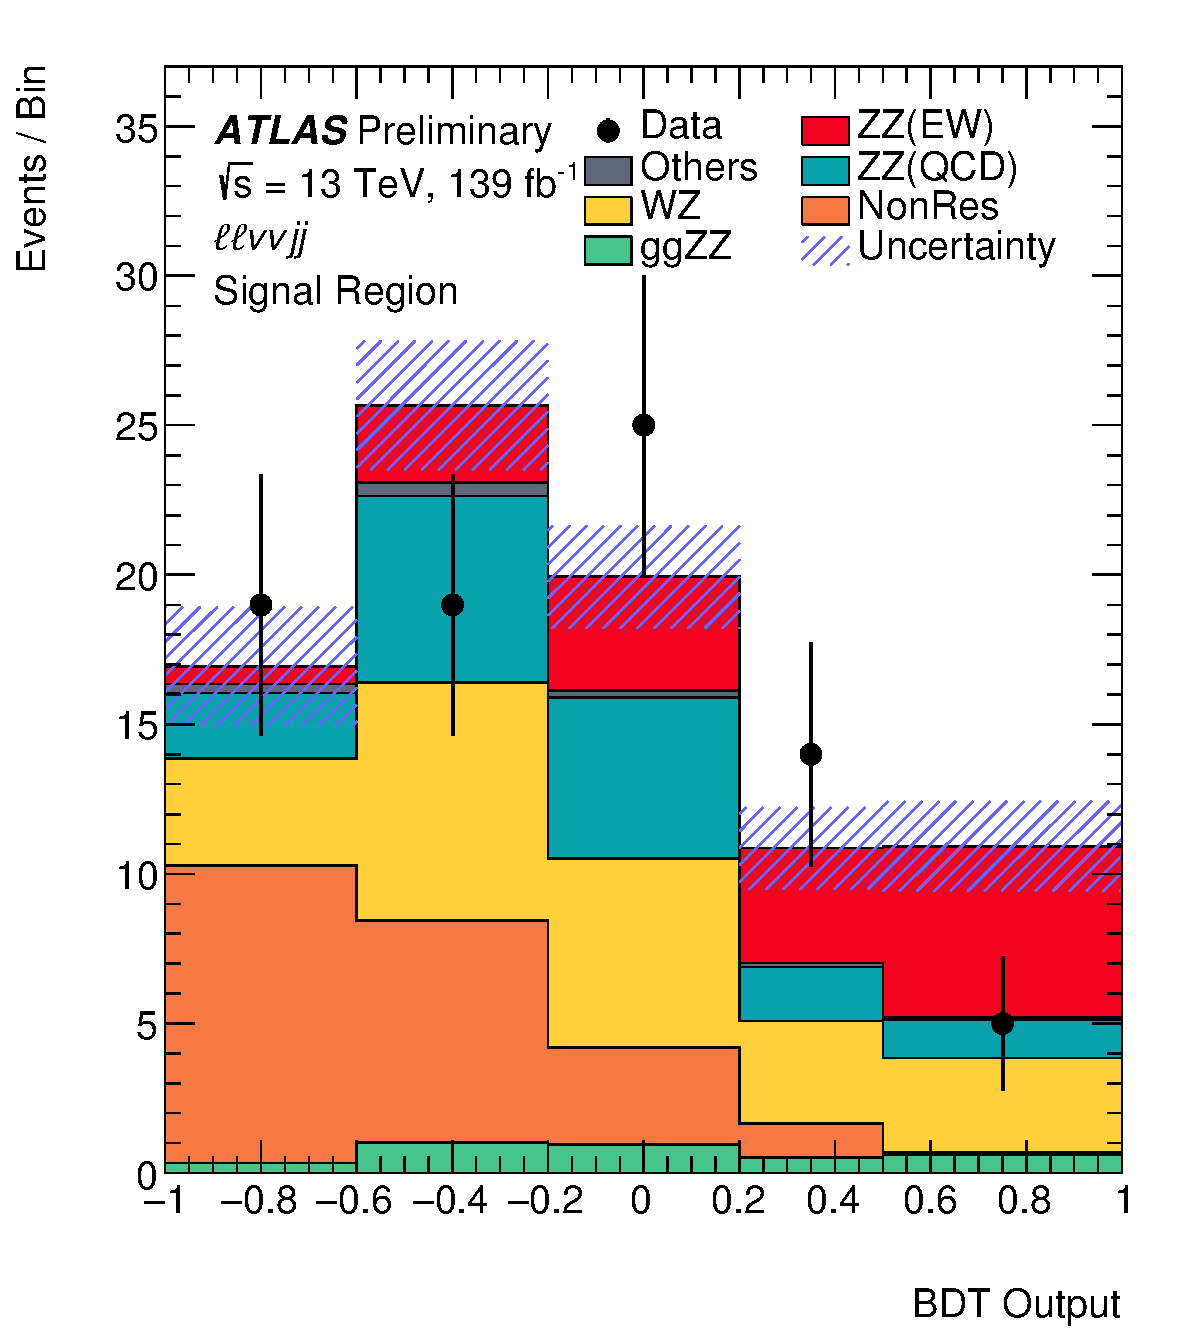
\includegraphics[width=0.325\textwidth]{figures/llvv/BDT_2l2v_SR_postFit_v1.pdf}\\
\end{center}
\caption{Observed and expected multivariate discriminant distributions after the statistical fit 
        in the \lllljj QCD CR (left), 
        and in the \lllljj (middle) and \llvvjj (right) signal regions.
        The error bands include the experimental and theoretical uncertainties, 
        as well as the uncertainties in \muEW and \muQCD.
        The error bars on the data points show the statistical uncertainty on data.
        }
\label{fig:MVA}
\end{figure}
